\documentclass{article}

% if you need to pass options to natbib, use, e.g.:
%     \PassOptionsToPackage{numbers, compress}{natbib}
% before loading neurips_2019

% ready for submission
% \usepackage{neurips_2019}

% to compile a preprint version, e.g., for submission to arXiv, add add the
% [preprint] option:
\usepackage[preprint]{neurips_2019}

% to compile a camera-ready version, add the [final] option, e.g.:
%\usepackage[final]{neurips_2019}

% to avoid loading the natbib package, add option nonatbib:
% \usepackage[nonatbib]{neurips_2019}

\usepackage[utf8]{inputenc} % allow utf-8 input
\usepackage[T1]{fontenc}    % use 8-bit T1 fontsa
\usepackage{hyperref}       % hyperlinks
\usepackage{url}            % simple URL typesetting
\usepackage{booktabs}       % professional-quality tables
\usepackage{amsfonts}       % blackboard math symbols
\usepackage{amsmath}
\usepackage{nicefrac}       % compact symbols for 1/2, etc.
\usepackage{microtype}      % microtypography
\usepackage{subfig}
\usepackage{float}
\usepackage{adjustbox}
\usepackage{multirow}
\usepackage{multicol}

\title{Dynamic Behaviors in Coupled Neuron System from a Game-Theoretic Standpoint}

\author{%
  Avinash Kori\\
  Department of Engineering Design\\
  Indian Institute of Technology, Madras\\
  \texttt{koriavinash1@gmail.com} \\
}

\begin{document}

\maketitle

\begin{abstract}
This paper is concerned with the theoretical investigation of game theory concepts in analyzing the behavior of dynamically coupled oscillators. Here, we claim that the coupling strength in any neuronal oscillators can be modeled using the concepts from game theory. We formulate the game to describe the effect of mixed-strategy equilibrium on two neuron systems of Hopf-oscillator and later demonstrate the application of the same assumptions and methods to $N \times N$ neuronal network. We also demonstrate the effect of the proposed method on MNIST data to show the equilibrium split of neurons in $N \times N$ neuronal grid for all the digits in MNIST digits. A major outcome of the paper is a learning algorithm based on the utility function derived from game theory.
\\

\textbf{keywords: } {Computational-modeling, Decision-making, Game-Theory, Nash-equilibrium, Coupled-Oscillator}

\end{abstract}

\section{Introduction}
Humans, like many other primitive organisms, are made up of the complex neural system, which is the combination of a large number of neurons forming complex neural architecture. Individual neurons are the build the building blocks of these complex neural architectures. Many models for single neuron behavior have been proposed and studied, to understand the coupling and firing patterns of these neurons. These models are the set of differential equations derived from the Hodgkin-Huxley model \cite{hodgkin1952dual}. Some commonly used models are Hopf-field model \cite{wang2003hopf}, FitzHugh-Nagumo model \cite{fitzhugh1961impulses}, Van der pol Oscillator \cite{parlitz1987period}, and Morris-Lecar neuron model \cite{morris1981voltage}. These models can capture some behaviors of the biological neurons \cite{gu2001integer, koper1996experimental, gu2013experimental}, As described in \cite{tsumoto2006bifurcations} Morris-Lecar model can capture the behavior of the membrane potential exhibiting spiking, or bursting state by changing the external forced current. 

Biological neurons always interact with one another to process information. The coupling in-between the neurons can be a result of electrical or chemical synapses. At equilibrium these neurons behave in synchrony, which results in a rhythmic group movement of information \cite{varela2001brainweb, golomb1994clustering}. This rhythmic movement is the result of neural coupling \cite{varela2001brainweb}. Tuning these coupling patterns makes it challenging to analyze the dynamic behavior of the neurons.

Recently, game theory has gained some attention in the field of neuroscience \cite{schuster2010application}. For instance, Neuroeconomics is the field where the concepts from game theory are extensively used to understand the decision-making process in humans \cite{loewenstein2008neuroeconomics}. Game theory can be applied to a wide variety of fields to analyze decision-making strategies followed by players \cite{srivastava2005using}. In \cite{hampton2008neural}, the authors formulated a simple two-player strategy game and tried to correlate their model prediction with functional MRI (fMRI) data. Most behavioral game theory literature demonstrates that humans think strategically in a single game, but strongly considers the strategies of the opponent \cite{costa2001cognition}. 

Dynamic game theory has also gained attention in recent days. In a dynamic system (DS) games, the very act of a player changes the dynamics of the game \cite{akiyama2000dynamical}. DS games have an evolving system of differential equations as a game environment, and these games have temporal components, and players make decisions at every instant of time. Evolutionary game theory \cite{dawkins1983john} has also offered some similar concepts of using the temporal component in games.

Considering the beliefs as variable and updating the beliefs based on some learning is rarely incorporated in the games. In the context of this paper, we consider each and every neuron to be a player, and they are provided with the two different strategies which correspond to couple or not to couple with other neurons. The coupling terms if made as a learnable parameter, which is updated based on the player's utility.

\begin{figure}
 \centering
 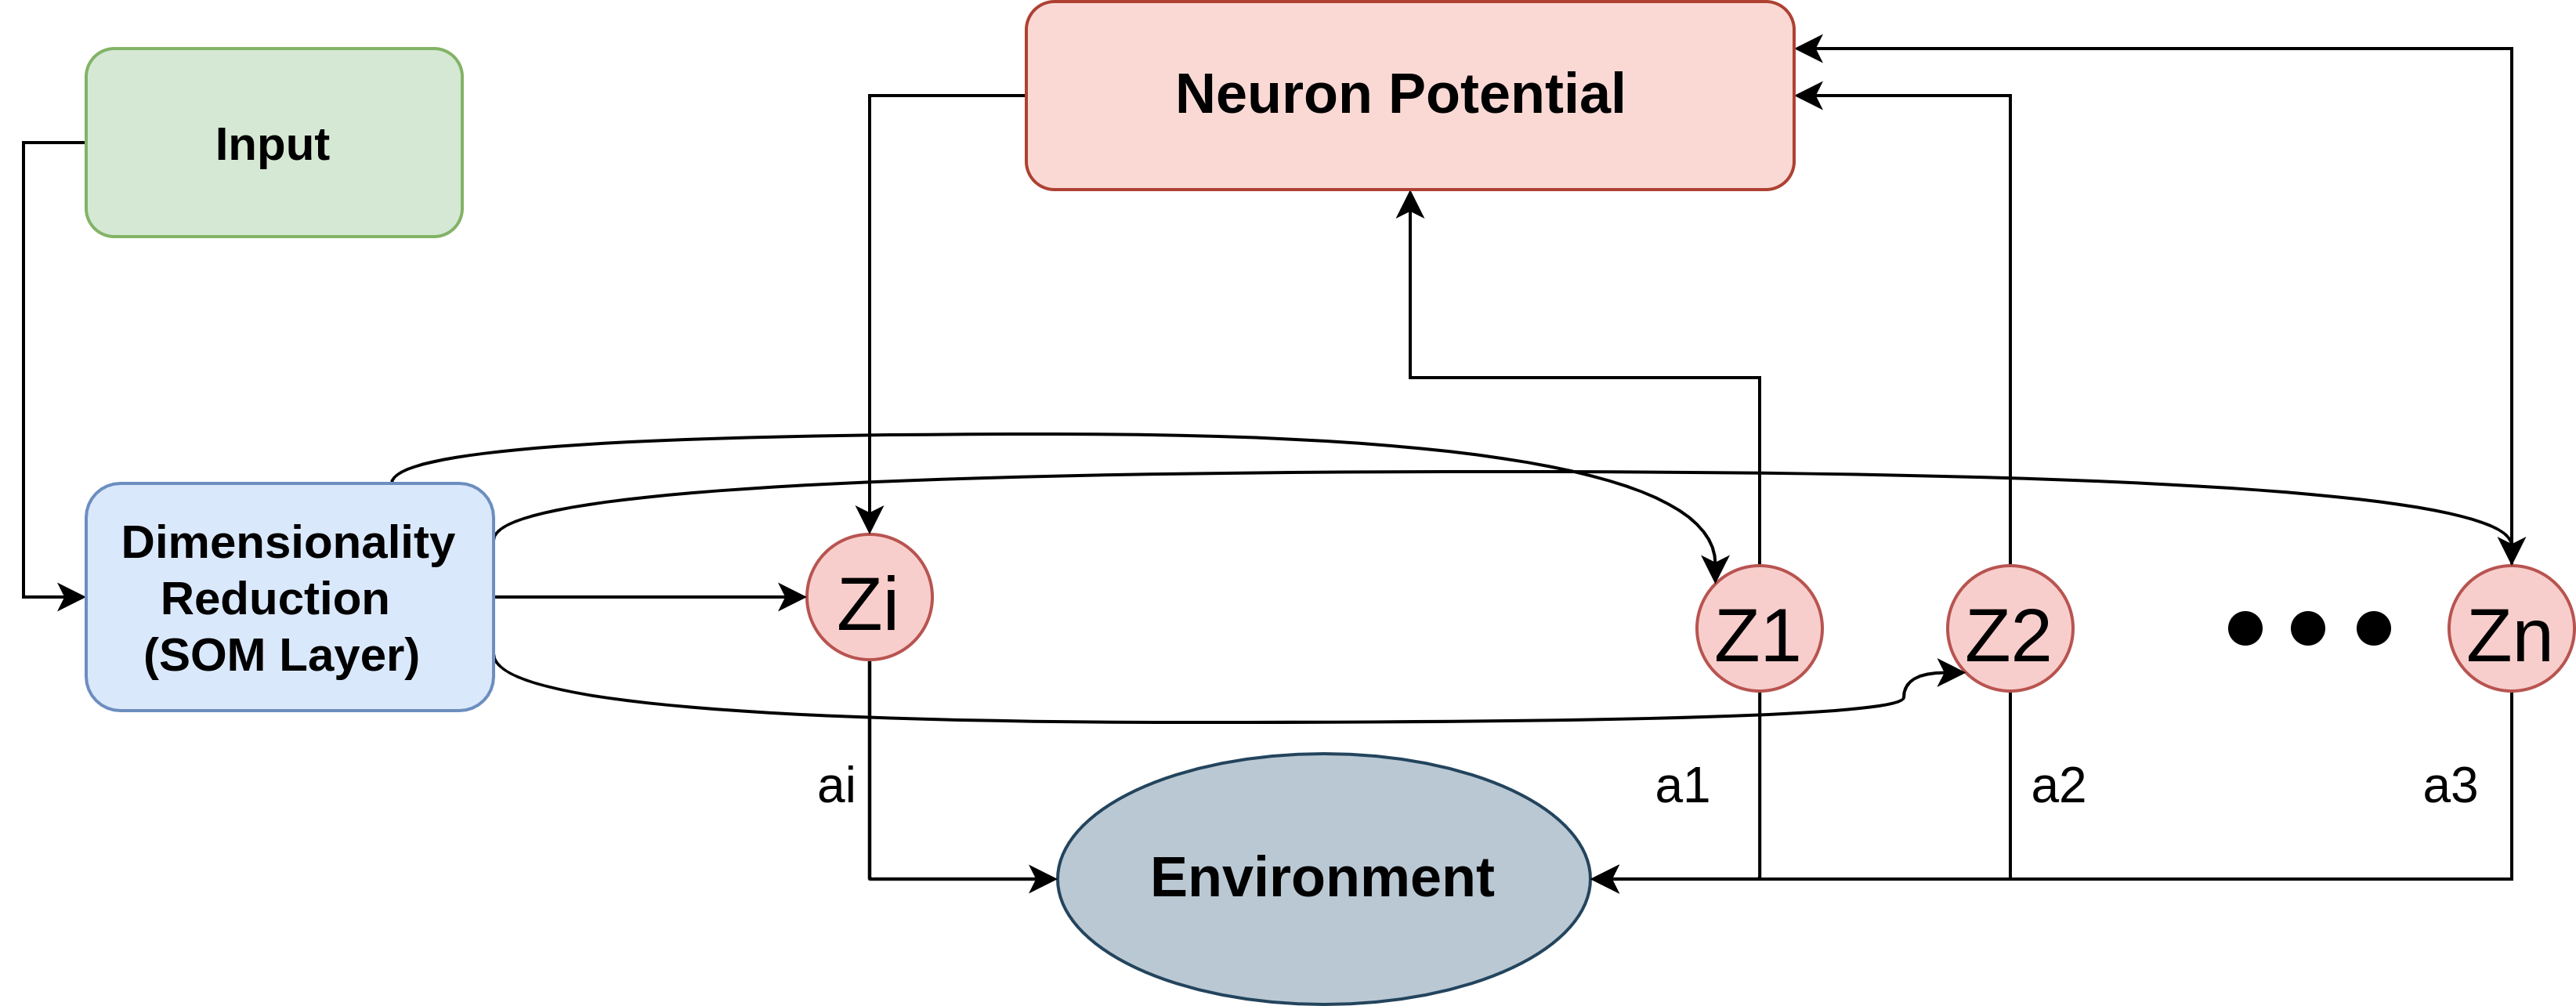
\includegraphics[width=1\textwidth]{overview.png}
 \caption{Above figure illustrates the proposed frame work. Input is random in case of two neuron framework, While it's MNIST digit in case of network example. Dimensionality reduction is SOM layer for network game, while it's identity block in case of two neuron game. ${Z_i}$ are neurons included in the game, $a_i$ is the action followed by the neuron (player) $i$, the selected action will affect the environment, the potential of the neuron will affect the firing of other neurons.}
 \label{fig: overview}
\end{figure}

Figure \ref{fig: overview} describes the overall structure of the proposed framework. In the remainder of this text, Section \ref{hpfosc} summarizes the Hopf-Oscillator and outlines circuit dynamics of the coupled neuron system. Section \ref{gameforintep} includes the game-theoretic formulation of the problem, also provides the interpretation of biological neurons. Section \ref{learning} summarizes the learning step and outlines its relation with game theory. Section \ref{exp} includes experimental details, followed by results and discussion in section \ref{resdis}. Section \ref{conc} ends the paper with conclusion.

\section{Hopf Coupled Oscillator}
\label{hpfosc}

As discussed previously, we'll be using Hopf oscillator for this work. Hopf oscillator is simplified Hodgkin-Huxley model, with just two parameters $\mu$ and $\omega$. Equation \ref{eqn: hopf} shows the single neuron Hopf oscillator, where $z \in \mathbb{C}$, $i = \sqrt{-1}$, and $\dot{z}$ indicates time derivative of complex variable $z$. This simple looking equation exhibits bifurcation property. Figure \ref{fig: stable} describes the convergence, divergence, stable state conditions of Hopf oscillator.

\begin{equation}
 \label{eqn: hopf}
 \dot{z} = (\mu - |z|^2)z + i\omega z
\end{equation}

\begin{figure}
 \centering
 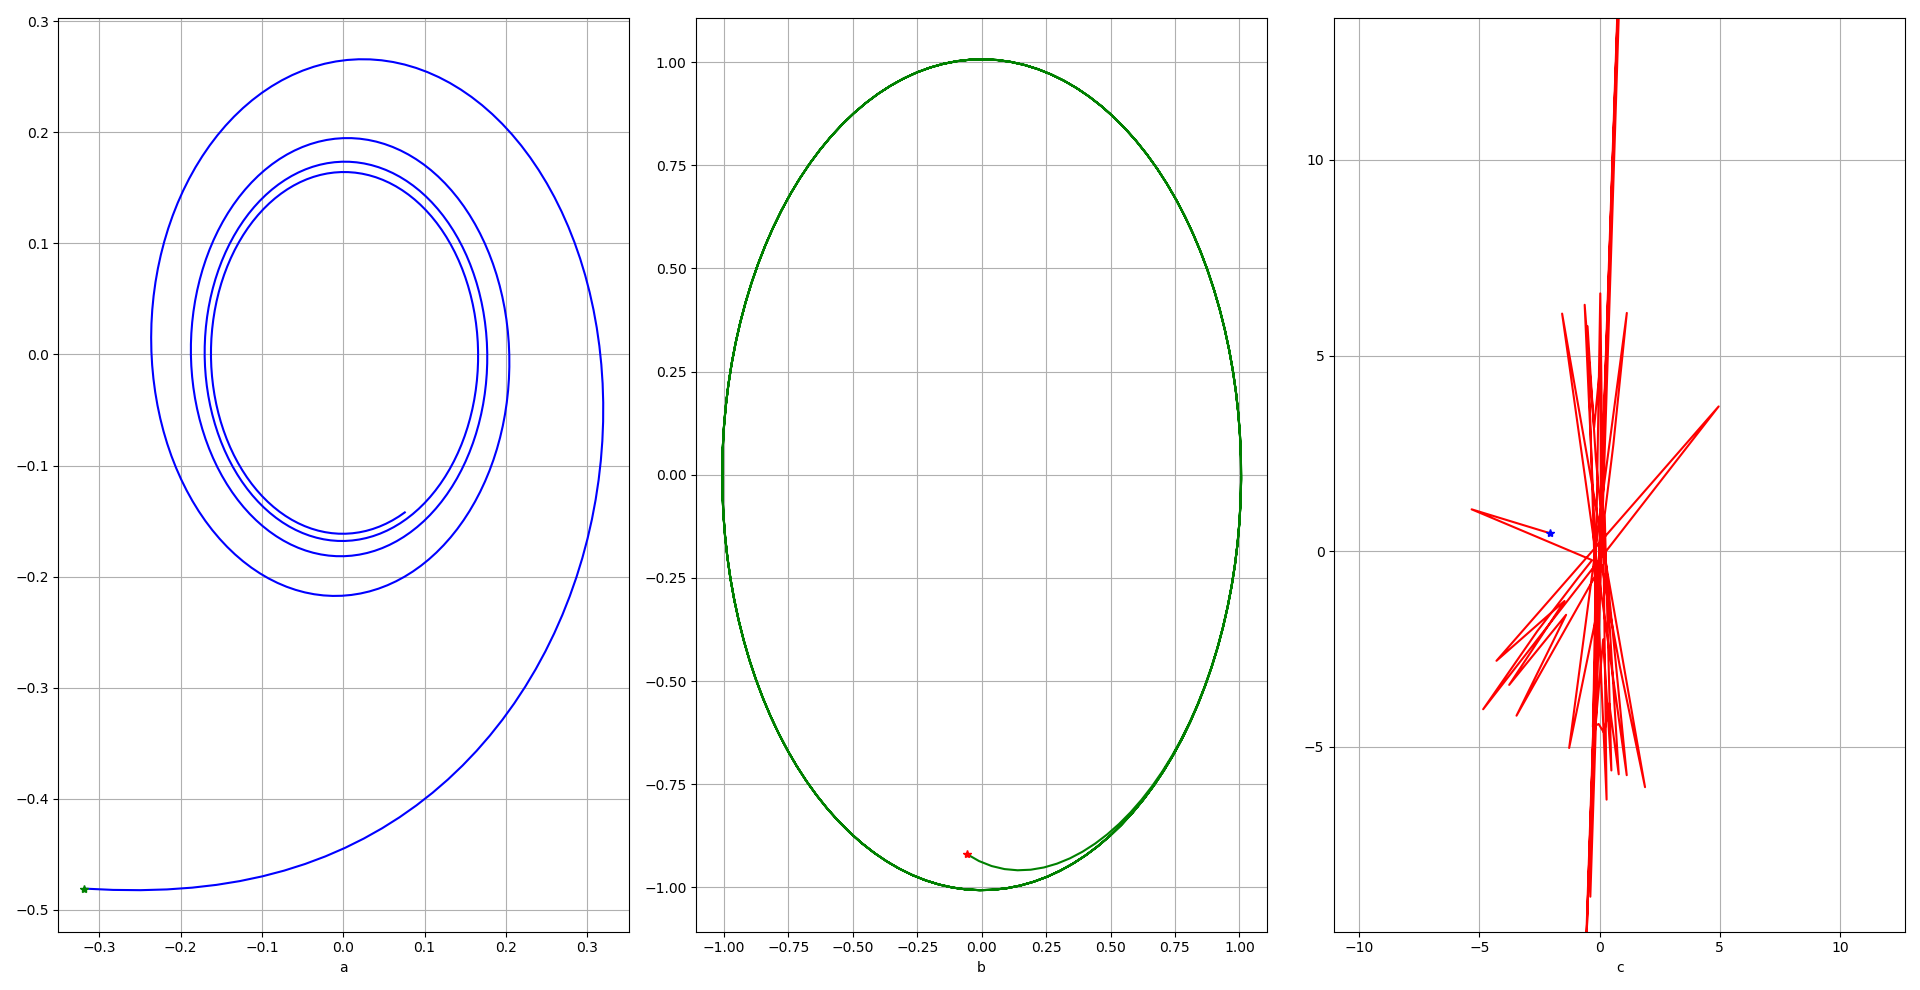
\includegraphics[width=1\textwidth]{hopf_initial.png}
 \caption{(a) Indicates the convergance of the system ($\mu = 0.1$), (b) Indicates the stable state of the system ($\mu = 1.0$), and (c) Indicates divergance criteria of the system ($ \mu = 15$). In all the expirements above $\omega = \frac{\pi}{6}$, $dt = 0.1$, and $*$ indicates the randomly initialized starting point.}
 \label{fig: stable}
\end{figure}

\begin{figure}
 \centering
 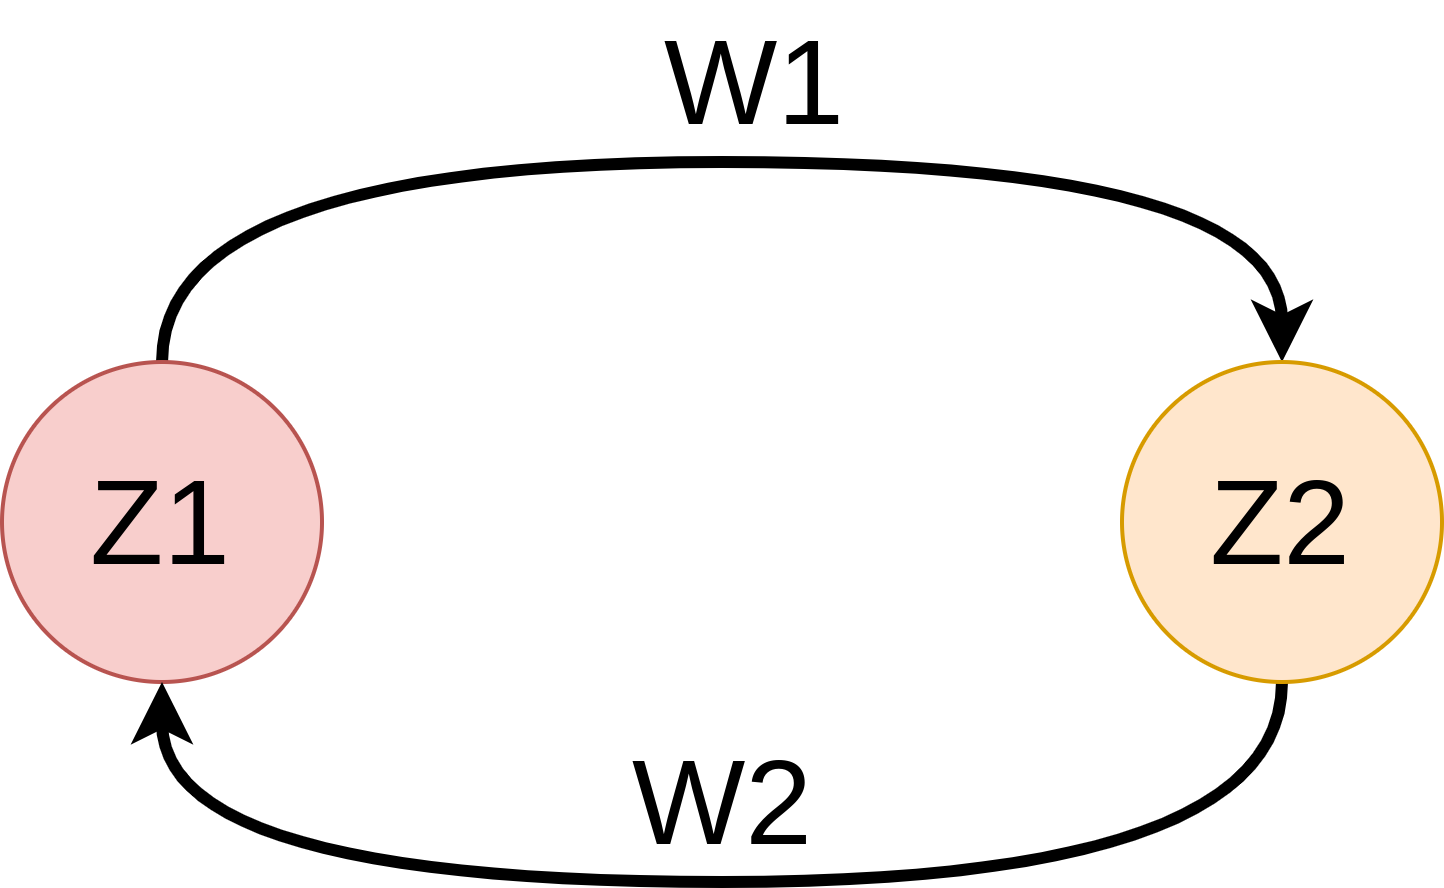
\includegraphics[width=0.3\textwidth]{two_neurons.png}
 \caption{$z_1$ and  $z_2$ indicates two different neurons, $W_1, W_2$ indicates the coupling factors for $z_2$ and $z_1$}
 \label{fig: two_neurons}
\end{figure}

In this work, for the formulation, we make use of a coupled neuron system with two neurons. Figure \ref{fig: two_neurons} describes the coupling between two neurons. Let $z_1, z_2$ be two different neurons; the activity of one is to get coupled with another neuron. Equation \ref{eqn: copuled_hopf} describes the coupled neuron system, where $W_1, W_2 \in \mathbb{C}$ captures interdependent coupling factor. 

\begin{subequations}
\label{eqn: copuled_hopf}
\begin{align}
 \dot{z_1} = (\mu - |z_1|^2)z_1 + i\omega z_1 + W_1 z_2 \\ 
 \dot{z_2} = (\mu - |z_2|^2)z_2 + i\omega z_2 + W_2 z_1 
\end{align}
\end{subequations}

By considering, eular form representation of complex numbers (i.e $z = re^{i\theta}$ and $W = Ae^{i\phi}$) and seperating real and imaginary components, the imaginary part of above equations \ref{eqn: copuled_hopf} reduces to equation \ref{eqn: copuled_hopf_eular_img} and real part reduces to equation \ref{eqn: copuled_hopf_eular_real} 

\begin{subequations}
\label{eqn: copuled_hopf_eular_img}
\begin{align}
 \dot{\theta_1} = \omega + \frac{r_2}{r_1} A_1sin(\phi_1 + (\theta_2 - \theta_1)) \\ 
 \dot{\theta_2} = \omega + \frac{r_1}{r_2} A_2sin(\phi_2 - (\theta_2 - \theta_1)) 
\end{align}
\end{subequations}

\begin{subequations}
\label{eqn: copuled_hopf_eular_real}
\begin{align}
 \dot{r_1} = (\mu - |r_1|^2)r_1 + r_2 A_1cos(\phi_1 + (\theta_2 - \theta_1)) \\ 
 \dot{r_2} = (\mu - |r_2|^2)r_2 + r_1 A_2cos(\phi_2 - (\theta_2 - \theta_1)) 
\end{align}
\end{subequations}

Let ($\psi = \theta_2 - \theta_1$, $r = r_2 - r_1$), at equilibrium $\dot{\psi} = 0$,and $\dot{r} = 0$ due to syncronization property followed by biological neurons as described in \cite{varela2001brainweb, golomb1994clustering}.

\begin{figure}
 \centering
 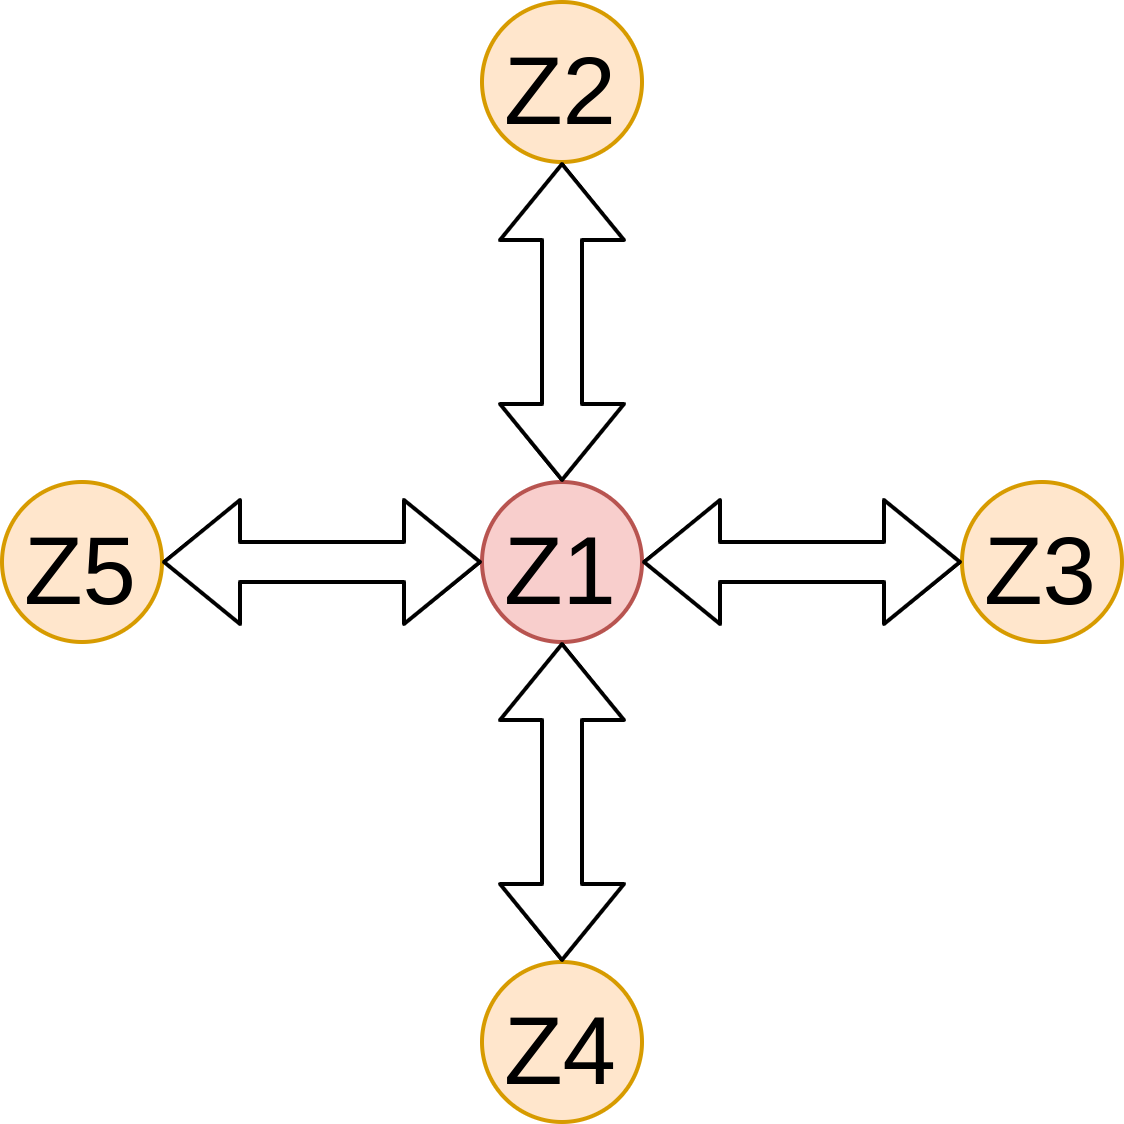
\includegraphics[width=0.3\textwidth]{network.png}
 \caption{$\{z_i\}$ indicates 5 different neabouring neurons in a network, there exist 2 couple factor inbetween every two neurons}
 \label{fig: network_neurons}
\end{figure}

\section{Self Organizing Map (SOM)}

\begin{figure}
 \centering
 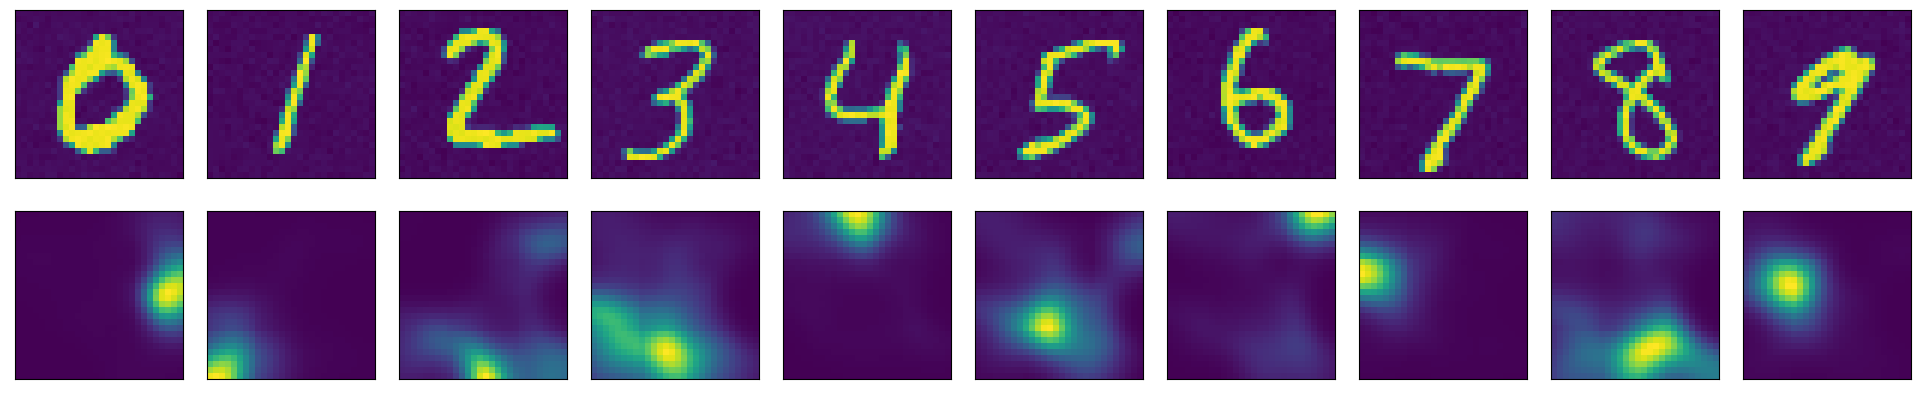
\includegraphics[width=1.\textwidth]{som_response.png}
 \caption{SOM response on MNIST handwritten digits; top row indicates MNIST test digits and bottom row indicates SOM responses for the given input data}
 \label{fig: som_response}
\end{figure}
The proposed network game uses Self-organizing Map (SOM) model as proposed by Kohonen \cite{}, whcih accounts for several key features of MNIST hand written digits \cite{}, these features are further used by neural sheet for further steps. SOM is type of unsupervised learning framework used for dimensionality reduction. In our case we use SOM to reduce the dimensionality of MNIST data from $(28\times28)$ to $10\times10$. The SOM was trained with MNIST hand written digits, Once trained the responses of SOM layer for any hand written digits is described in figure \ref{fig: som_response}, we make use of these responses with key features for our further analysis.

\section{Game Theoretic Formulation and Interpretations}
\label{gameforintep}

In order to appreciate and fully understand forthcoming sections, it's important to brief about different games and also layout the proposed structure mathematically. For this work, we formulate this coupling game as a strategic form game. As in this game, we assume that the decisions of both the players are independent and non-cooperative in nature. Figure \ref{fig: two_neurons}, indicates the both players involved: $N = \{Neuron-1, Neuron-2\}$, strategies possible for both the players are: $s_i = \{Couple(C), Don't-Couple(DC)\}$. The neuronal potential to mapped to strategies as described in equation \ref{eqn: potential_strat}. Strategy set ${s_1}$ and ${s_2}$, will result in total $s_1 \times s_2$ strategies. In this case all the strategies are: $\{\{C, C\}, \{C, DC\}, \{DC, C\}, \{DC, DC\}\}$. As biology encourages synchrony, we model the utilities accordingly; the payoff matrix in figure \ref{fig: payoff} describes the same.
In the payoff matrix in figure \ref{fig: payoff}, using the definitions of rationality and common knowledge, the game can be reduced to an equilibrium point where both the players find coupling as the most advantageous action (strategy set $\{C, C\}$). 

\begin{equation}
  \label{eqn: potential_strat}
  s_i =
    \begin{cases}
      C & \text{if $|z_i^t| > 0.5$}\\
      DC & \text{otherwise}\\
    \end{cases}       
\end{equation}


\begin{figure}
 \centering
 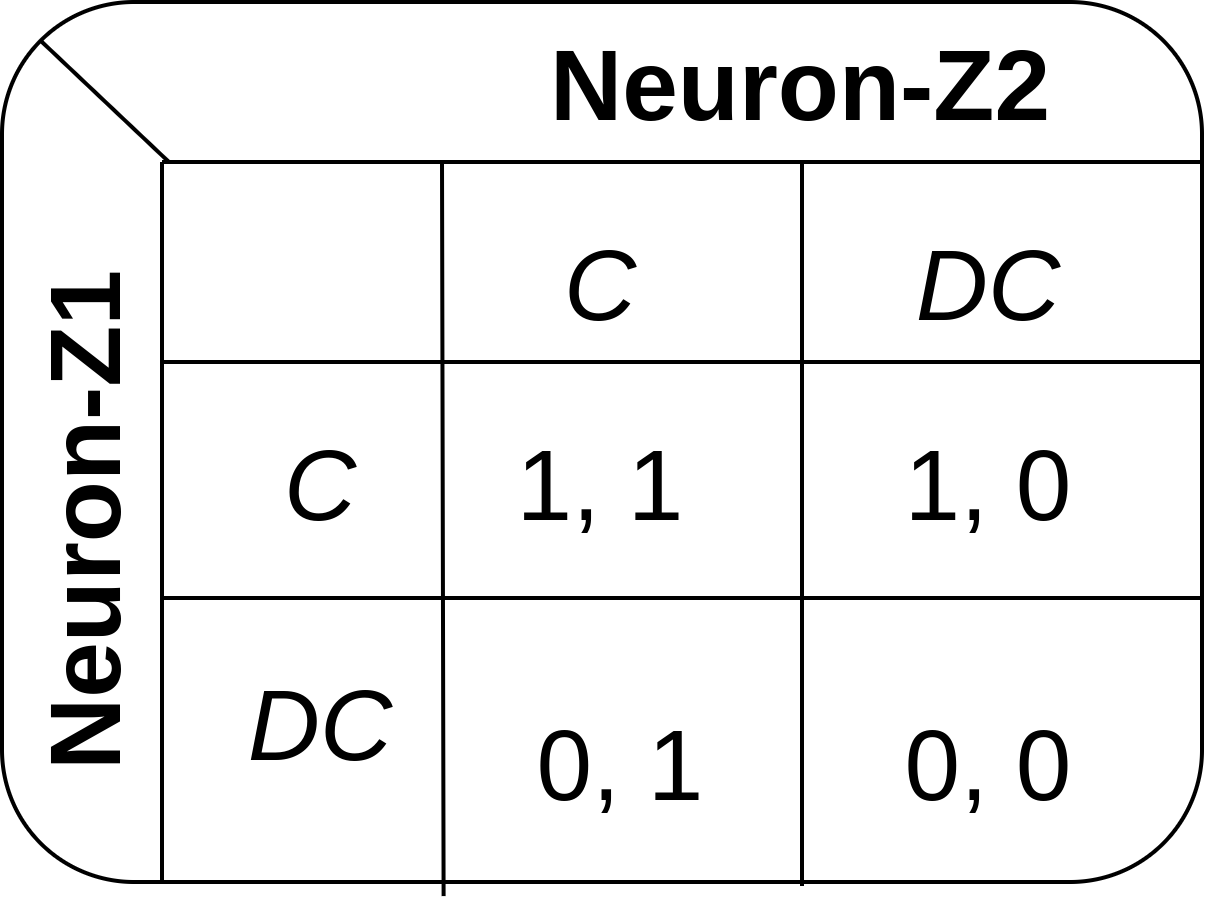
\includegraphics[width=0.3\textwidth]{payoff.png}
 \caption{C}
 \label{fig: payoff}
\end{figure}

\textit{Payoff Matrix:} Is used to map set of strategies to there utilities, where utility function is a mapping from strategy space to real-valued number ($u_i: \{s_1 \times s_2\} \rightarrow \mathbb{R}$). In this paper, we modeling coupling as a game, figure \ref{fig: payoff} describes the payoff matrix for this game. As synchronization can be observed from biological neurons, we provide a higher payoff for the player willing to a couple.   

\textit{Common Knowledge:} Common Knowledge is information that is the same and known by all the players. In the formulated game as any player at any point of time know the utilities and all the strategies of other player, which makes it complete information game. (Every player knows all the possible strategies of other player, but not the exact strategy what the opponents play)

\textit{Rationality:} Economists and mathematicians invoke arguments about "rational" behavior to explain the behavior of players based on given circumstances \cite{bicchieri2004rationality}. These assumptions can be considered as building blocks in game theory. One of the assumptions of rationality is that the player never plays a strategy, which provides less payoff when compared to other strategies in certain external circumstances.

\textit{Equilibrium:} Is a point in the game where every player selects a strategy and fix to that strategy irrespective of other players. At this state, no player finds it advantages to switch strategy if the strategies of the other players remain unchanged. The set of strategies at this state is considered as equilibrium strategies, More commonly referred to as Nash Equilibrium \cite{holt2004nash}.

\textit{Rationality and equilibrium in the above game:} Based on the rationality assumption discussed above, both the players find it optimal to follow the coupling strategy, which results in Pure Strategy Nash Equilibrium at strategy set $\{C, C\} $. Again by rationality assumptions, it can be easily seen that the strategy set $\{C, C\}$ also survives Iterative Elimination of Strictly Dominated Strategies (IESDC) \cite{narahari2014game}. 

\textit{How does a player's action affect the environment?} As the considered game is dynamic in nature, which means the game itself may converge, diverge, or remain in a stable state based on a player's actions. Because of this changing environment, to ensure constant coupling, we can have a dynamic payoff matrix or learnable parameter associate with coupling terms, which adjusts the coupling parameter and maintain the environment in the desired state.

\section{Learning}
\label{learning}

As discussed in the above section, we have an additional learnable parameter associated with the coupling variable to maintain the environment in the desired state. The most commonly used learning rule for neurons is Hebbian learning \cite{kempter1999hebbian}. Hebbian learning is a neuroscientific theory which is inspired by the biological neural synaptic adjustment mechanism. Hebbian learning tries to explain both functional and structural plasticity in biological neurons \cite{song2000competitive}. Here, in this work, we make use of the modified Hebbian method, which considers utilities of the neuron along with neuron state in update rule, as described in equation \ref{eqn: modified_hebbian}. Where $\Delta W^t_i$ is the weight update for player $i$s coupling variable at that instant $t$, $u_i$ denotes the utility of player $i$, $W^t$ indicates the coupling variable at instant $t$, $z^t$ is neuron potential at instant $t$, and $z^{t*}$ is conjugate neuron potential.  

\begin{equation}
 \label{eqn: modified_hebbian}
 \Delta W^t_i = - W^t_i + (u_i(s_1, s_2) + 1)z^t_{i}z^{t*}_{-i}
\end{equation}

\textit{Equilibrium theoretical analysis:} 
Once the system achieves equilibrium, $\Delta W^t_i$ will remain 0, which results in $W^t_i = (u_i(s_1, s_2) + 1)z^t_iz^{t*}_{-i}$.

Converting to Euler form will result in: $A^t_i e^{i\phi^t_i} = (u_i(s_1, s_2) + 1) r^t_ie^{i\theta^t_i} r^t_{-i}e^{i\theta^t_{-i}}$, using update terms for both the neurons simultaniously we get equation \ref{eqn: ampli_relation}
\begin{equation}
\label{eqn: ampli_relation}
\frac{A_1^t (u_2(s_1, s_2) + 1)}{A_2^t (u_1(s_1, s_2) + 1)} = e^{i(\phi_2 - \phi_1 - 2\psi)}
\end{equation}
By comparing both the sides we can say that $\phi_2 - \phi_1 - 2\psi = n\pi$, since there's no imaginary component on left side of the above equation. This phase difference makes the ratio of amplitude of coupling weights propotional to the ratio of utilities as described in equation \ref{eqn: utility_apli}.
\begin{equation}
\label{eqn: utility_apli}
\frac{A_1^t}{A_2^t} = \frac{u_1(s_1, s_2) + 1}{u_2(s_1, s_2) + 1}
\end{equation}
Theoretical coupling to strategies relation is described in the table \ref{tab: ampli_relation}
\begin{table}
  \caption{Coupling strength based on player strategies}
  \label{tab: ampli_relation}
  \centering
  \begin{tabular}{lll}
    \toprule
    $s_1$     & $s_2$     & $\frac{A^t_1}{A^t_2}$ \\
    \midrule
    $C$       & $C$       & 1   \\
    $C$       & $DC$      & 2   \\
    $DC$      & $C$       & 0.5   \\
    $DC$      & $DC$      & 1   \\
    \bottomrule
  \end{tabular}
\end{table}



\section{Expirements}
\label{exp}

\textit{Two Neuron model:} First, to validate the formulated game, we demonstrate the behavior of the neuronal system due to coupling and the above utility form. Here, we randomly initialize the potential for $z_1$ and $z_2$ and use numerical methods and modified Hebbian rule to drive neuronal potential to an equilibrium point.

\textit{Network Extention:} We perform this experiment, to demonstrate the formulated game on the network of $N\times N$ neurons, where each neuron is connected to its adjacent 4 neurons as described in figure \ref{fig: network_neurons}. We use SOM responses to initialize these neurons and again use numerical methods along with modified Hebbian rule to achieve equilibrium. In this experiment, the aim is to observe different equilibrium coupling phases for different digits in the dataset. The system of equations defining the network game and the corresponding Hebbian rule is described in equations \ref{eqn: multi_neuron} where $Nbr_{z_k}$ denotes neighboring neurons, which are directly connected to $z_k$.

\begin{subequations}
\label{eqn: multi_neuron}
\begin{align}
 \dot{z_k} = (\mu - |z_k|^2)z_k + i\omega z_k + W_k \prod_{p \in Nbr_{z_k}} p \\ 
 \Delta W_k = - W_k + (u_k(s_k, s_{-k}) + 1)z_k \prod_{p \in Nbr_{z_k}}p^*
\end{align}
\end{subequations}

\section{Results and Discussion}
\label{resdis}
\begin{figure}[h]
    \centering
    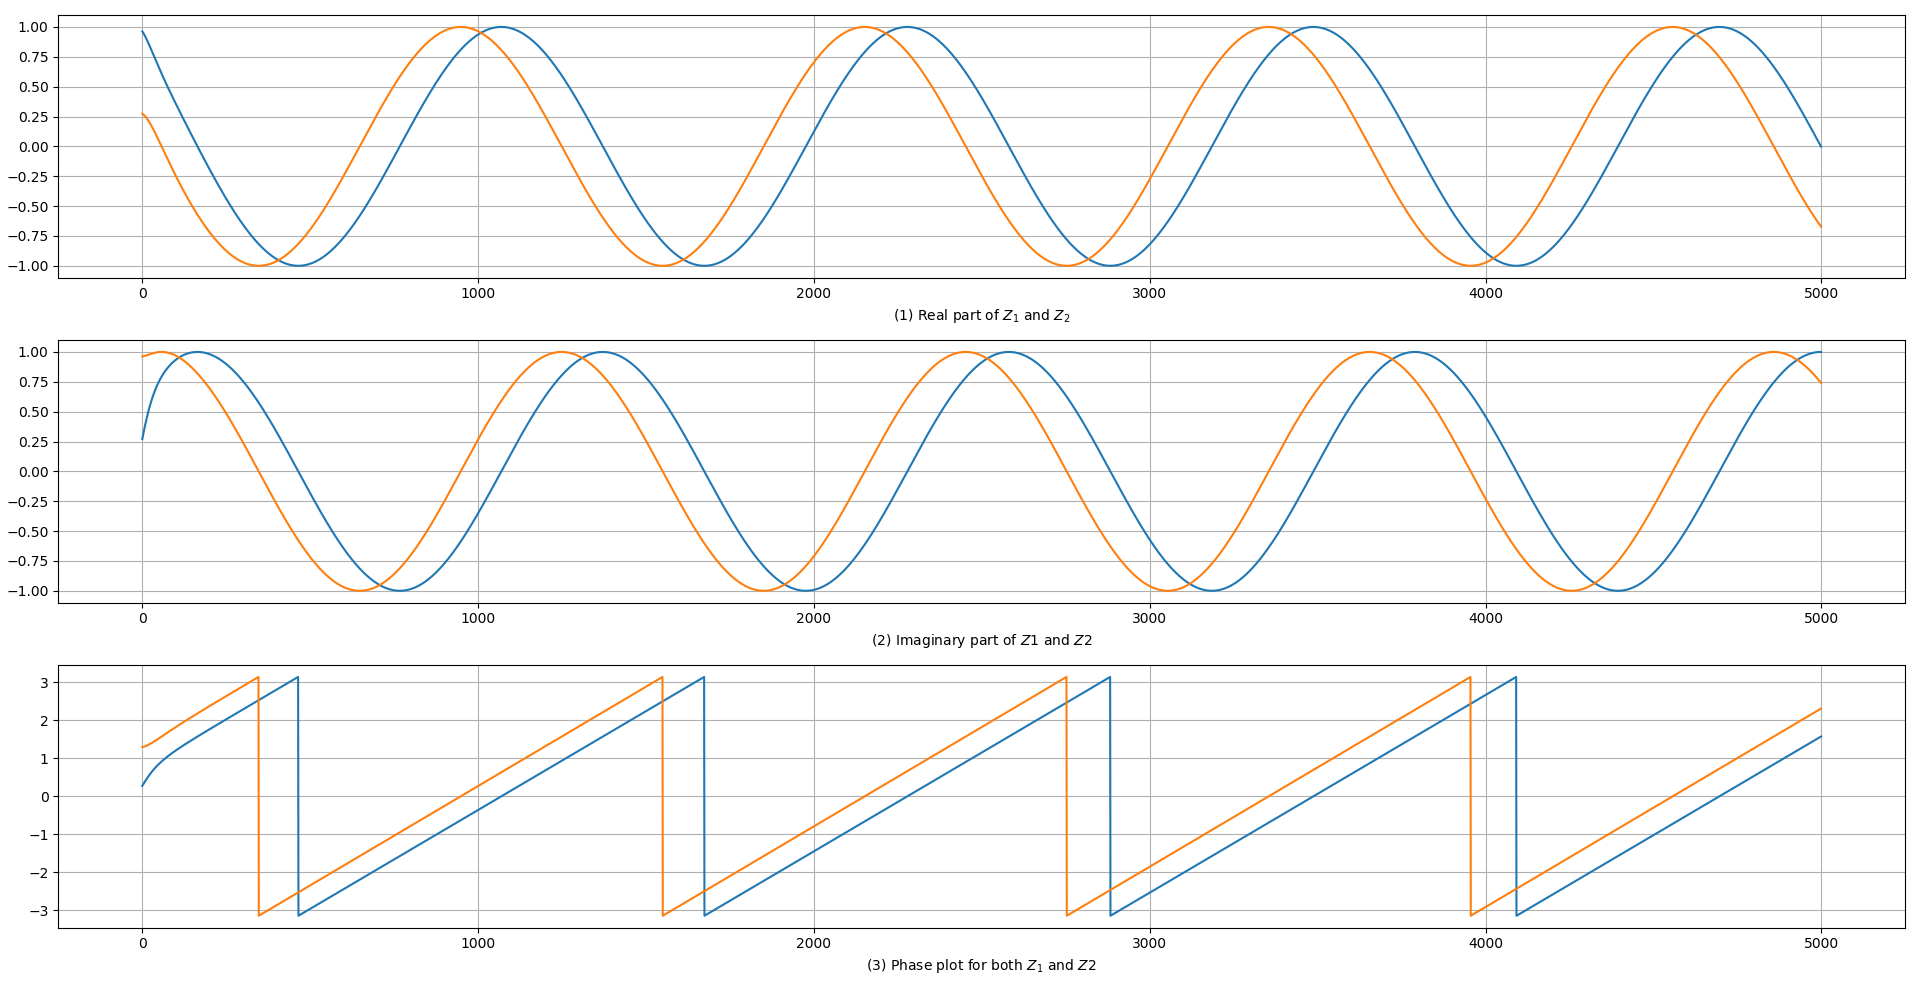
\includegraphics[width=1.\textwidth]{two_neuron_phase_potential.png}
    \caption{Results for two neuron model}
    \label{hist_exp}
\end{figure}
\section{Conclusion}
\label{conc}
The paper provides a novel concept for formulating the neuron coupling as a game, to our knowledge, this the first time neural coupling is formulated using a game-theoretic framework. In the paper, we also demonstrate the modified Hebbian rule for learning coupling parameters and demonstrate the results on a network and two neuron frameworks. The proposed method is tested on Hopf oscillator but can be easily extended to any other oscillators. These findings are further correlated with biological neuronal behavior in terms of synchronization and synaptic strength development.  

\subsubsection*{Acknowledgments}

The author gratefully acknowledges the discussions with Dr. Srinivas Chakravarthi on neural circuitry, and Dr. Puduru Viswanandha Reddy on the concepts of game theory.

\bibliographystyle{unsrt}
\bibliography{ref.bib}

\end{document}
